\documentclass{article}
\usepackage{amsmath}
\usepackage{amsfonts}
\usepackage{hyperref}
\usepackage{enumitem}
\usepackage{graphicx}

\title{DBRP Research Paper}
\author{}
\date{}

\begin{document}

\maketitle

\section{Task 1 - DBRP}

\subsection*{Goal}
\begin{itemize}
    \item Gain understanding on bulk reconstruction algorithm
    \item Source: Discrete bulk reconstruction, Scott Aaronson and Jason Pollack
\end{itemize}

\section{Background}

\subsection{AdS (Anti-de Sitter)}
\begin{itemize}
    \item Higher-dimensional \textbf{bulk} space
    \item \textbf{Bulk}: AdS space
    \item \textbf{Surface}: Geometric object within AdS space
    \item \textbf{Minimal area}: Surface that spans the boundary subregion and has the smallest possible area \textit{(RT surface in AdS/CFT)}
    \item The bulk is very hard to calculate directly because of quantum gravity, therefore perform calculations on CFT.
\end{itemize}

\subsection{CFT (Conformal Field Theory)}
\begin{itemize}
    \item \textbf{Boundary} $\Rightarrow$ CFT
    \item Lower-dimensional space that forms "edge" or "boundary" of AdS bulk
    \item Non-gravitational theory that lives on the boundary of the AdS spacetime
    \item Information of boundary is encoded in the bulk
\end{itemize}

\subsubsection*{Quick Notes about AdS and CFT}
\begin{itemize}
    \item If dealing with 5-dimensional AdS bulk, the boundary is typically 4-dimensional, and the CFT lives on this 4-dimensional boundary.
    \item DBRP idea in physic terms:
    \begin{itemize}
        \item Because the CFT is a non-gravitational theory, it is easier to make computations and to understand. And because it lives on the boundary of the AdS space, we can use the CFT to reconstruct the gravitational dynamics of the AdS bulk.
        \item Given a CFT state, we can determine the corresponding spacetime that the CFT describes, including its geometry and gravitational dynamics.
        \item Then we can use entanglement entropy in the CFT to learn about spacetime geometry in the bulk.
    \end{itemize}
\end{itemize}

\subsection{AdS/CFT}
\begin{itemize}
    \item \textbf{AdS/CFT correspondence} $\Rightarrow$ The gravitational theory in the bulk is equivalent to the non-gravitational CFT on the boundary
    \item i.e. Two theories describe the same physics, but from different perspectives
    \item \textbf{Holographic Relationship}: Everything happening in the bulk AdS spacetime can be described by the boundary CFT, and vice versa
    \item Consists of two theories (theory of quantum gravity and a quantum field theory, with no gravity). The relation between the two theories is called "holographic".
    \item Theories are "equivalent"? (yet to be proven)
    \item Meaning, there exists a mapping or "dictionary" that maps all states and observables from one theory to corresponding states and observables in the other
    \item Currently lack a full dictionary for the AdS side
\end{itemize}

\subsubsection*{Quick note about spacetime geometry (physics)}
\begin{itemize}
    \item Gravity is a curvature of spacetime (caused by mass and energy)
    \item "Geometry" of spacetime refers to this curve:
    \begin{itemize}
        \item If no gravity, geometry is simple and uncurved
    \end{itemize}
\end{itemize}

\subsubsection{Spacetime Geometry for AdS/CFT}
\begin{itemize}
    \item In AdS space, geometry is negatively curved.
    \item \textbf{CFT can reconstruct the geometry of AdS bulk}: Meaning, data in the CFT can be used to determine how spacetime is shaped or curved in the AdS bulk.
    \item \textbf{Entanglement is directly related to geometry of the bulk spacetime}: 
    \begin{itemize}
        \item Amount of entanglement in different regions of CFT tells us about structure and curvature of the corresponding bulk spacetime in AdS.
        \item More entanglement on the boundary implies more curvature or structure in the bulk geometry.
        \item Proven with RT formula: more entanglement = larger minimal surface area = more curved and intricate bulk geometry.
    \end{itemize}
\end{itemize}

\subsubsection*{Why important?}
\begin{itemize}
    \item Shape of spacetime tells us how gravity behaves.
    \item If we can reconstruct the bulk geometry from the CFT, we can gain insights into the quantum aspects of gravity and understand how measurements (or experiments) on the boundary affect the information encoded in the bulk.
\end{itemize}

\subsection{Entanglement Measurements}
\begin{itemize}
    \item Not needed for DBRP because problem states initially given full AdS/CFT correspondence.
\end{itemize}

\subsubsection*{Von Neumann entropy}
\begin{itemize}
    \item Refers to a measure of quantum entanglement, i.e., information contained in a specific region (usually in lower-dimensional CFT).
\end{itemize}

\subsubsection*{Ryu-Takayanagi (RT) Formula and Holographic Dictionary}
\begin{itemize}
    \item Key entry in holographic dictionary is \textit{Ryu-Takayanagi (RT) formula}.
    \item Equates von Neumann entropy of subregion of boundary state with the minimal area among all bulk surfaces that end on that boundary region.
    \item Meaning: Entropy (amount of quantum information) in a certain part of the boundary is tied to the area of the smallest surface that stretches into the bulk but connects to that boundary (geometrical way of understanding quantum entanglement).
\end{itemize}

\subsubsection*{Minimal area of bulk surface}
\begin{itemize}
    \item In higher-dimensional bulk space (AdS) exists a surface whose area corresponds to entanglement in boundary region.
    \item Theory says: Smallest possible area of this surface (RT surface) is proportional to entropy of boundary subregion.
    \item Meaning: If you can find RT, you know the entropy (or information) of the subregion inside the boundary.
    \item The more entangled the boundary region is, the larger the area of corresponding surface in the AdS bulk.
\end{itemize}

\textbf{RT surface is proportional to von Neumann entropy which quantifies quantum entanglement or information of subregion.}

\section{Discrete Bulk Reconstruction Problem}
Official statement initialization:
\[
\mathcal{H} = \otimes^{N}_{i=1}\mathcal{H}_{i}
\]
\begin{quote}
    Note about tensor product, Hilbert space, and qubits:
\end{quote}
\begin{itemize}
    \item Tensor Product is a mathematical operation used to describe a system with multiple qubits. It combines two or more Hilbert spaces into a single composite Hilbert space, or one large vector space. The larger space captures the full state space of the combined quantum system.
    \item For a single qubit: $|0\rangle$, $|1\rangle$ form a basis for a two-dimensional Hilbert space.
    \item Therefore, an $n$-qubit system has a Hilbert space of dimension $2^n$.
\end{itemize}

\subsubsection*{Min-Cut Theory}
\begin{itemize}
    \item Feature of AdS/CFT.
    \item Given a finite weighted undirected graph \( G \) with real edge weights \( w(e) \geq 0 \), as well as two disjoint vertices \( R, R' \), a min-cut is a set \( C \) of edges with minimum total weight
    \[
    W = \sum_{e \in C} w(e)
    \]
    whose removal disconnects \( R \) from \( R' \).
\end{itemize}

\section{Problem Set-Up}
Can model the bulk by a weighted undirected graph where each subregion is an RT (or minimal area) surface, which corresponds to min-cuts in \( G \).

\begin{center}
    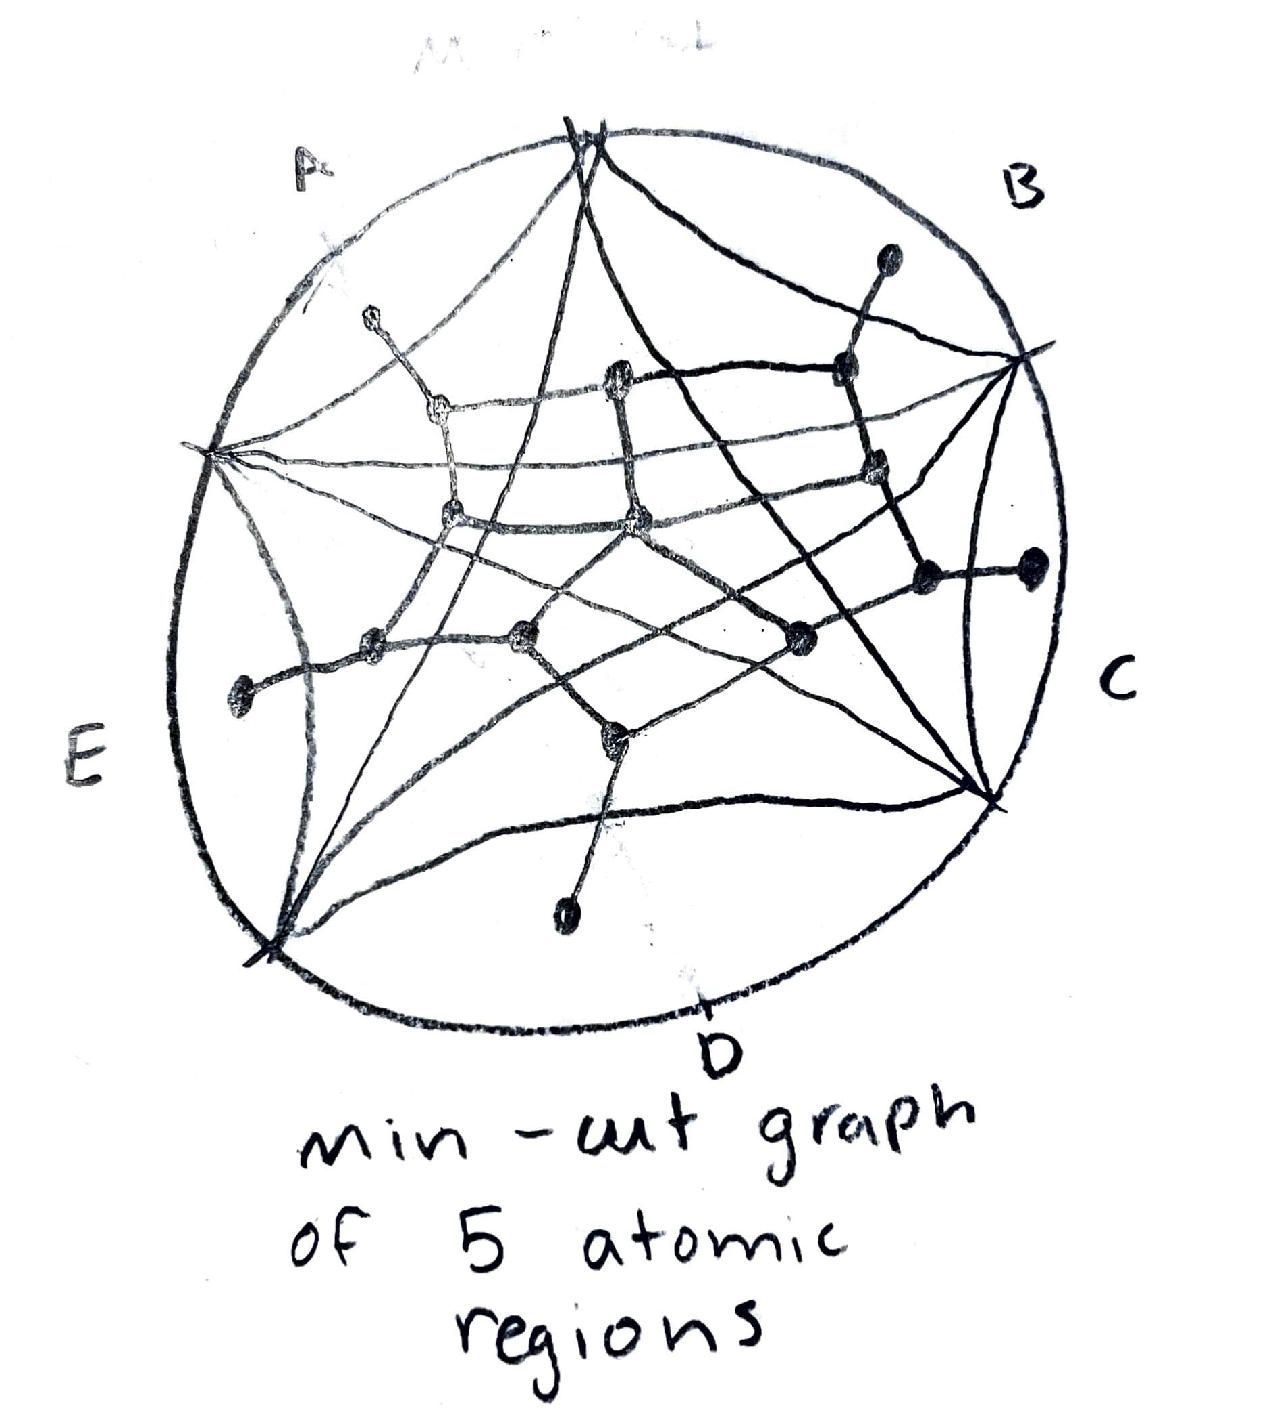
\includegraphics[width=0.8\textwidth]{min_cut_graph.pdf}
\end{center}

\subsection{Official Statement}
Given as input a list of atomic boundary regions labeled \( 1, \dots, N \), a list of subsets of the regions \( R_1, \dots, R_k \subseteq [N] \), and a real-valued entropy \( S(R_i) \geq 0 \) for each \( R_i \), the weight of the minimum cut separating \( R_i \) from the rest of the boundary vertices (i.e., from \( [N] - R_i \)) is equal to \( S(R_i) \).

\subsection{General Idea}
\begin{itemize}
    \item If we are given the complete entanglement structure of the boundary, we are therefore provided with a min-cut graph of the boundary entropies. We can then perform an experiment in the bulk space and use min-cut theory on the boundary to reconstruct the entropy graph.
\end{itemize}

\textbf{This is basically the inverse min-cut problem.} Given the min-cut, find the graph that gave you the min-cut solution. 

\section{Required Properties}
To ensure a solution exists we \textbf{need} the following properties:

\begin{enumerate}
    \item \textbf{Subadditivity (SA)}: entropy of \( A \) plus entropy of \( B \) is \( \geq \) entropy of \( A \cup B \)
    \[
    S(A) + S(B) \geq S(AB)
    \]
    \begin{center}
        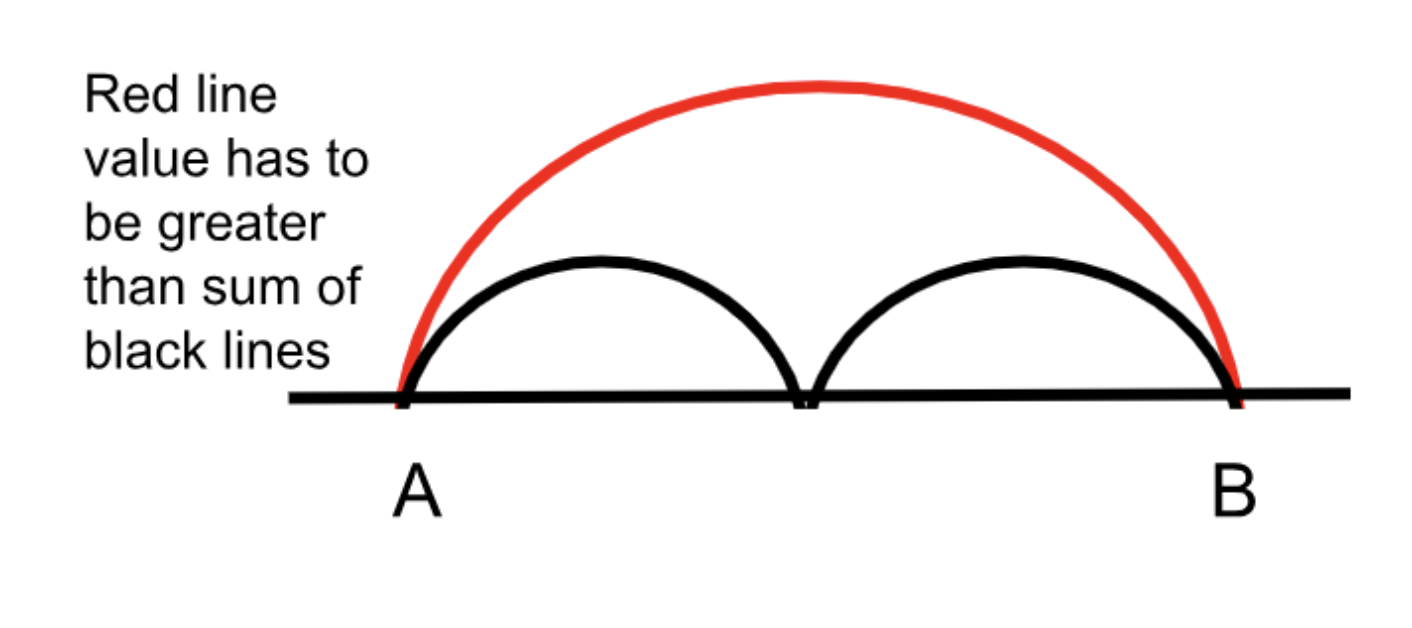
\includegraphics[width=\linewidth]{subaddivity.png}
    \end{center}
    
    \item \textbf{Strong Subadditivity (SSA)}
    \[
    S(AB) + S(BC) \geq S(B) + S(ABC)
    \]
    \begin{center}
        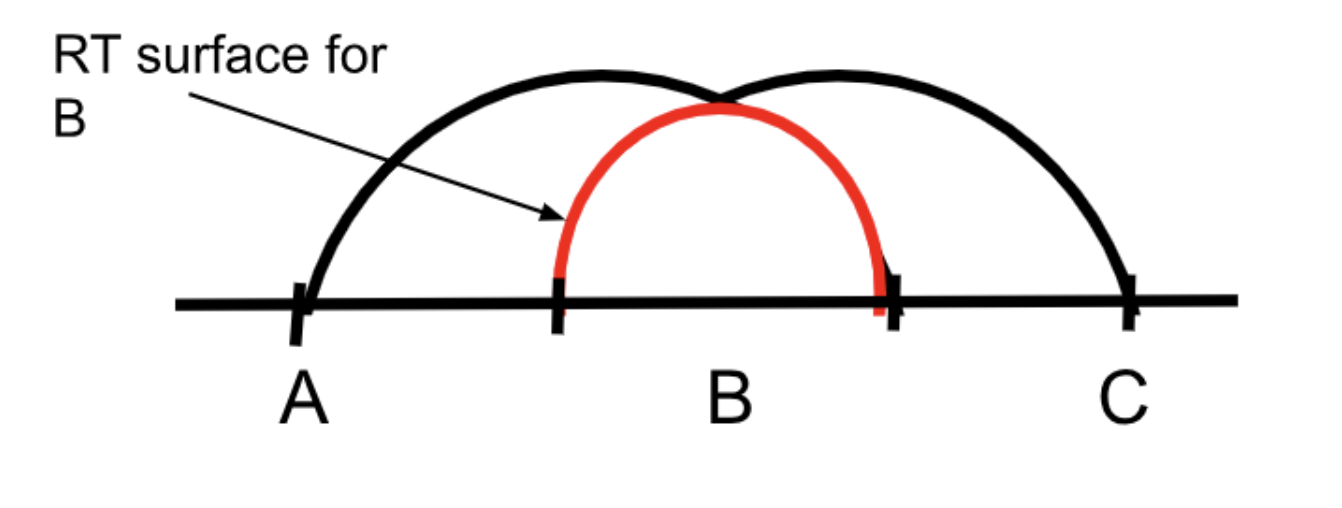
\includegraphics[width=0.8\textwidth]{strong_subaddivity.png}
    \end{center}
\end{enumerate}

\section{Holographic Quantum State}
\begin{itemize}
    \item Boundary state in CFT that, due to holography, has a corresponding interpretation in bulk AdS space.
    \item This allows us to perform computations on a lower-dimensional boundary with no gravity, which then gives us information about higher-dimensional gravity in bulk space.
    \item Note: Entanglement entropy of a region in boundary can correspond to the area of the minimal surface in the bulk (RT-formula).
\end{itemize}

All holographic quantum states \textbf{must} satisfy the following property:
\begin{itemize}
    \item \textbf{Monogamy of Mutual Information (MMI)}
    \[
    S(AB) + S(BC) + S(AC) \geq S(A) + S(B) + S(C) + S(ABC)
    \]
\end{itemize}

\textbf{Question:} Are these properties what give us geometry?

\section{DBRP on 1-dimensional Hilbert Space}
\begin{itemize}
    \item Note: To perform DBRP on a higher-dimensional Hilbert space, take the tensor product of each Hilbert space to create one large Hilbert space.
    \[
    \mathcal{H}_{\text{total}} = \mathcal{H}_1 \otimes \mathcal{H}_2 \otimes \dots \otimes \mathcal{H}_N
    \]
    \item Upper bound for contiguous boundary regions: 
    \[
    \frac{N(N-1)}{2}
    \]
    \item Can specify \textit{all} \( 2^N \) non-contiguous entropies in terms of \( \frac{N(N-1)}{2} \) contiguous entropies.
    \item Formula is minimum of 2 different possibilities:
    \[
    S(AC) = \min\{ S(A) + S(C), S(B) + S(D) \}
    \]
    \begin{center}
        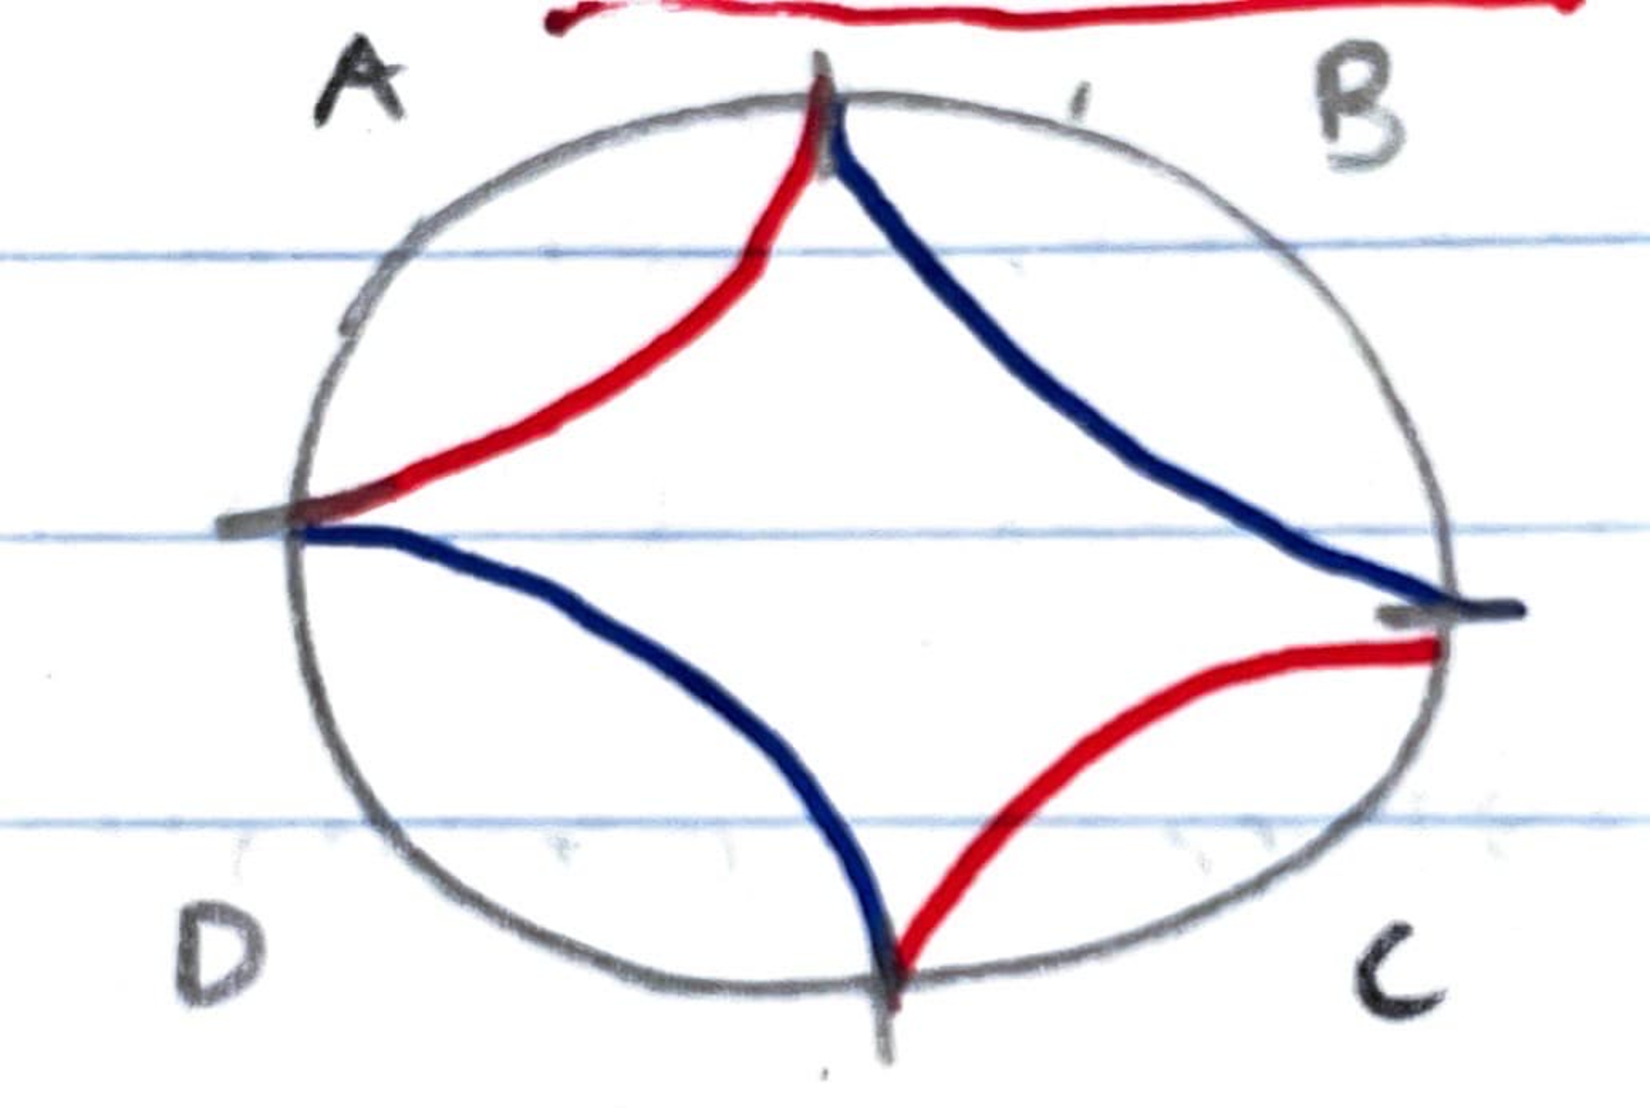
\includegraphics[width=0.8\textwidth]{parts.pdf}
    \end{center}
\end{itemize}


\section{Theorem: 1D Boundary}
In special cases of a 1D boundary divided into \( N \) parts, given contiguous entropies satisfying SSA, we can always find a graph model of the bulk in linear time \( O(N^2) \). The graph model is planar, universal, and has \textbf{only} \( O(N^2) \) vertices.

\textbf{Note:} Only need to satisfy SSA for 1D.

\section{Proof of 1D, with Examples}
\begin{itemize}
    \item Any contiguous boundary data that satisfies SSA admits a "bulkless" graph.
    \item A bulkless graph is a graph of pure edges and no vertices.
    \item After creating a bulkless graph, we can solve for what the edge weights should be! By using a system of linear equations, SSA ensures nonnegativity.
\end{itemize}


\begin{center}
    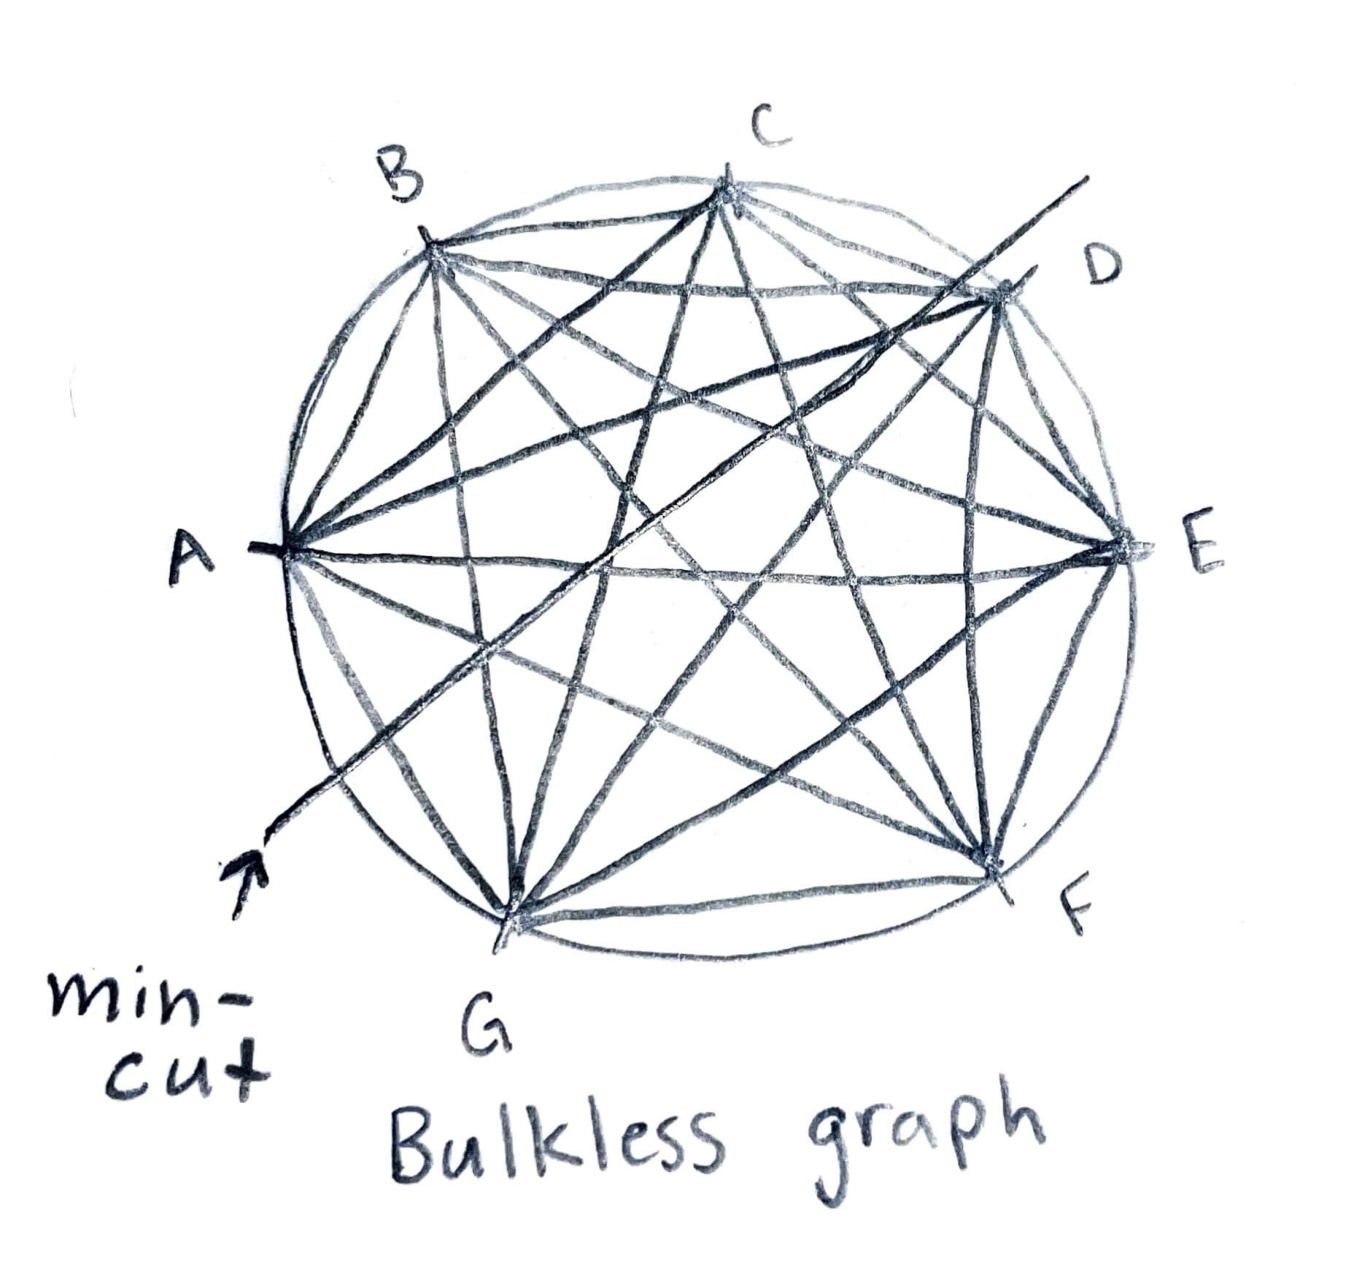
\includegraphics[width=0.8\textwidth]{bulkless_graph.pdf}
\end{center}

This will lead to a planar graph model of the bulk. The next step will be to get the model...

\section{Chord Construction}
\begin{itemize}
    \item Get model of graph.
    \item Take all edges in between atomic boundary regions and add a chord (vertex) where each edge intersects.
    \item Edge weights = weights from bulkless graph.
\end{itemize}


\begin{center}
    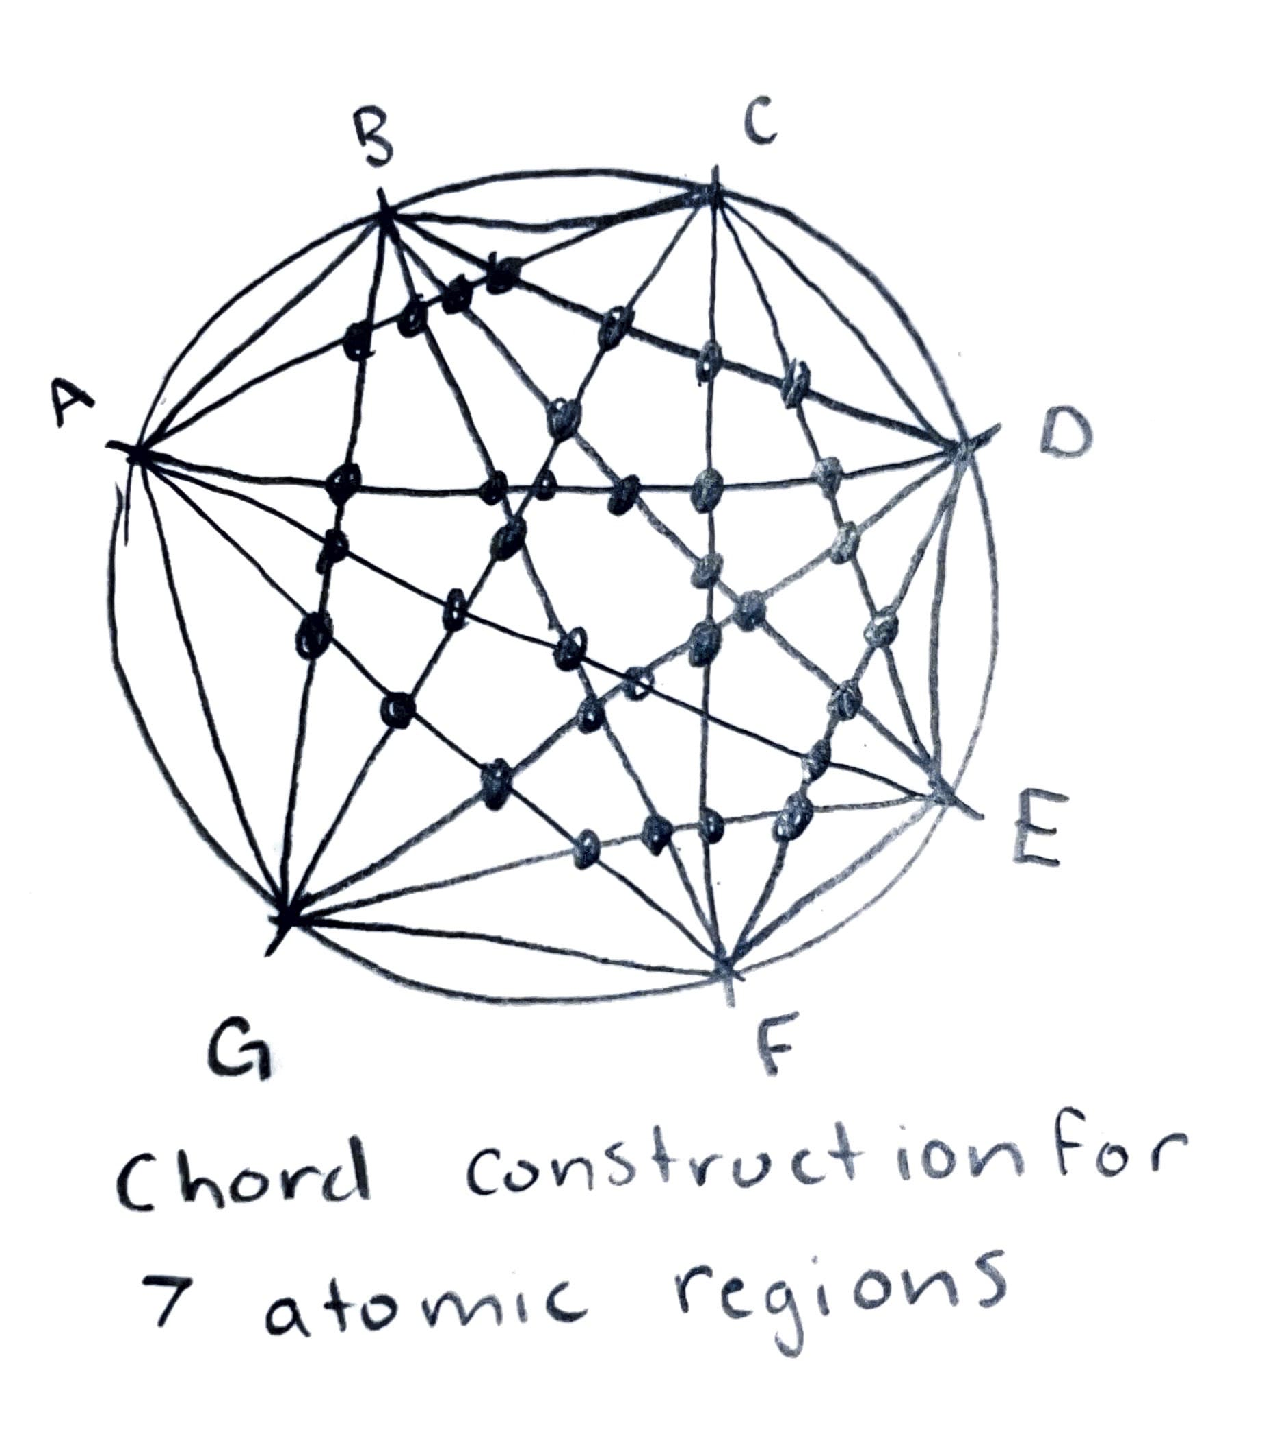
\includegraphics[width=0.8\textwidth]{chord_construct.pdf}
\end{center}

This yields a planar graph with \( O(N^4) \) vertices (not optimal) and the same cut structure as the bulkless graph.

\textbf{Note:} Since the bulkless graph has correct cut values, the planar graph will also have correct cut values. However, \( O(N^4) \) is not optimal, so a better construction was developed...

\section{Diamondwork Construction}
\begin{itemize}
    \item Yields \( O(N^2) \) vertices and edges.
    \item Reduce via a planar graph made up of "overlapping" triangles, each contributing weight from the bulkless graph.
    \item Overlapping triangles are minimal surfaces that cut deeper into the bulk.
    \item Add edge weights together to overlap them.
    \item Min-cuts cut the same as the bulkless graph.
\end{itemize}


\begin{center}
    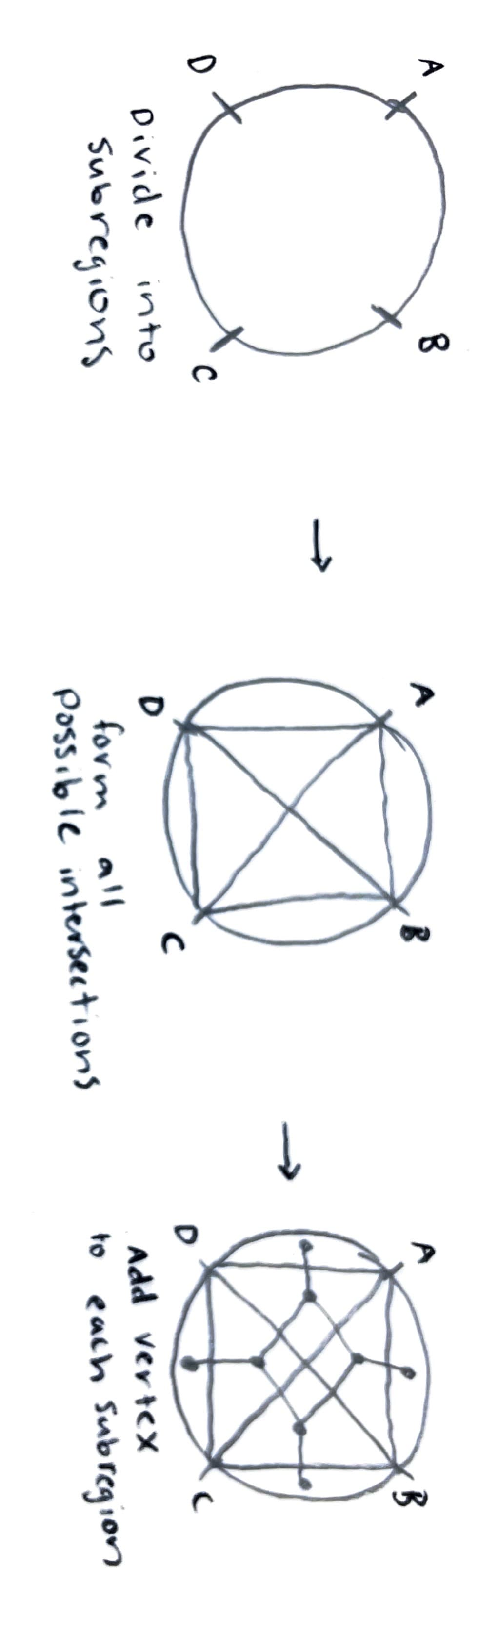
\includegraphics[width=0.8\textwidth]{subregions.pdf}
\end{center}

\section{Harmonic Edge Weights}
This is the discrete version of AdS geometry. The entropy of a length \( L \) boundary region (where \( L \leq N/2 \)) is given as:

\section{ADD PHOTO}
%\begin{center}
%    \includegraphics[width=0.8\textwidth]{https://hackmd.io/_uploads/B1S_4MBMJl.jpg}
%\end{center}

\section{Why No Black Holes?}
\begin{itemize}
    \item All edge weights have the same value, therefore the RT minimal surface means nothing.
    \item There is no advantage to cutting deeper into the bulk.
\end{itemize}

\section{ADD PHOTO}
%\begin{center}
%    \includegraphics[width=0.8\textwidth]{https://hackmd.io/_uploads/BJLSNo1VJe.jpg}
%\end{center}

\end{document}

